
%%%%%%%%%%%%%%%%%%%%%%%%%%%%%%%%%%%%%%%%%%%%%%%%%%%%%%%%%%%%%%%%%%%%%%

\documentclass{beamer}

% For more themes, color themes and font themes, see:
% http://deic.uab.es/~iblanes/beamer_gallery/index_by_theme.html
%
\mode<presentation>
{
  \usetheme{Madrid}       % or try default, Darmstadt, Warsaw, ...
  \usecolortheme{default} % or try albatross, beaver, crane, ...
  \usefonttheme{serif}    % or try default, structurebold, ...
  \setbeamertemplate{navigation symbols}{}
  \setbeamertemplate{caption}[numbered]
} 
\usepackage[utf8]{inputenc}
\usepackage[spanish]{babel}
\usepackage{chemfig}
\usepackage[version=3]{mhchem}
\PassOptionsToPackage{demo}{graphics}
\usepackage{pgfpages}
\usepackage{booktabs}
\pgfpagesuselayout{resize to}[%
  physical paper width=8in, physical paper height=6in]


\title[]{Caracterización computacional de algoritmo de segmentación de fuego y humo basado en redes neuronales convolucionales}
\author{Paola Yang}
\institute{UTFSM}
\date{\today}

\begin{document}

\begin{frame}
  \titlepage
\end{frame}


%\begin{frame}{Outline}
%  \tableofcontents
%\end{frame}

\section{Introducción }

\begin{frame}{Introducción}
	\begin{columns}
		\column{.4\textwidth}
        \begin{itemize}
        \item Los incendios forestales son un problema a nivel mundial y afectan significativamente al ecosistema y a la comunidad. 

        \end{itemize}
        
        \column{.6\textwidth}
	\begin{figure}[H]
	\centering
 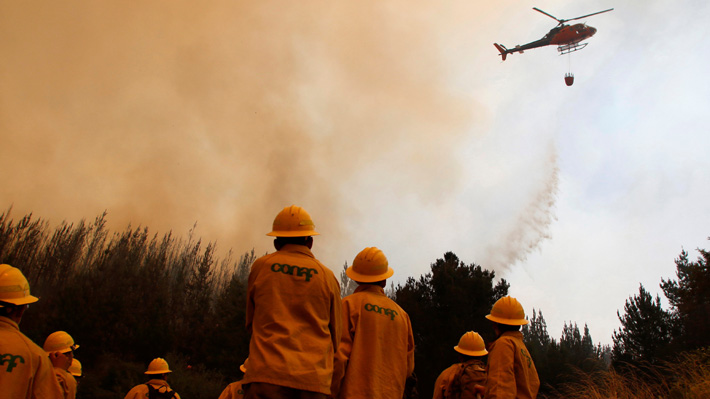
\includegraphics[width=1\textwidth]{fig/conaf.jpg}
	\end{figure}
	\end{columns}
\end{frame}




\begin{frame}{Introducción}
\centering
 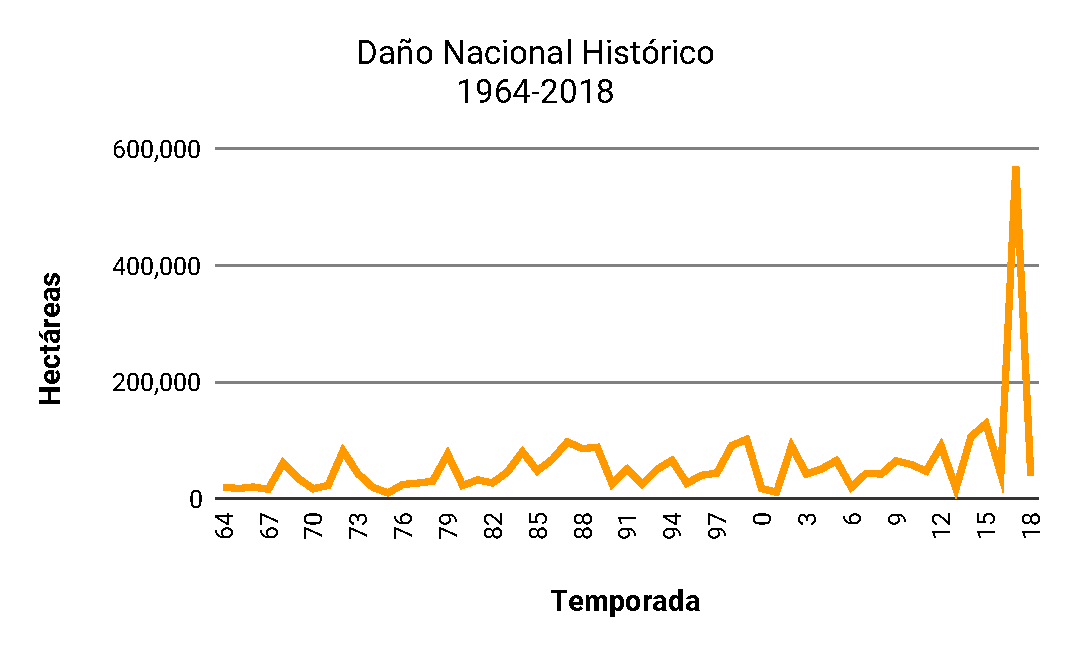
\includegraphics[width=0.8\textwidth]{fig/chart.pdf}
 \newline
 \begin{text}
En Chile, la superficie afectada por incendios forestales promedia las 57.000 hectáreas quemadas. 
\end{text}
\end{frame}











\begin{frame}{Wild Fire Watch}
	\begin{columns}
	
		\column{.4\textwidth}
        \begin{itemize}
        \item Monitoreo incendios a través de un sistema basado en drones. 
        \end{itemize}
        
        \column{.6\textwidth}
	\begin{figure}[H]
	\centering

        %
\includegraphics[width=0.1\textwidth]{fig/WFW.png}
        
 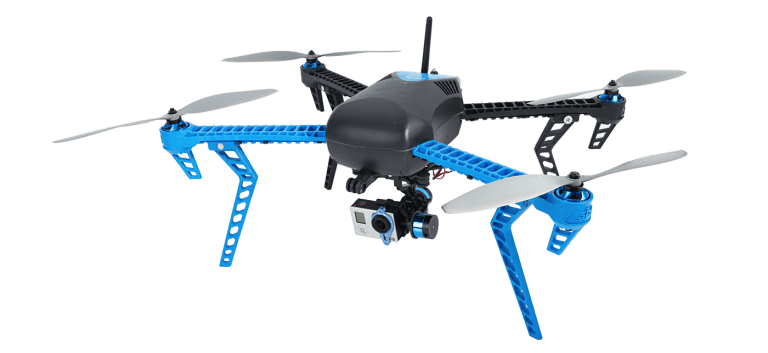
\includegraphics[width=1\textwidth]{fig/iris.png}
	\end{figure}
	\end{columns}
\end{frame}



\begin{frame}{Modelo de segmentación de fuego y humo}

	\centering
 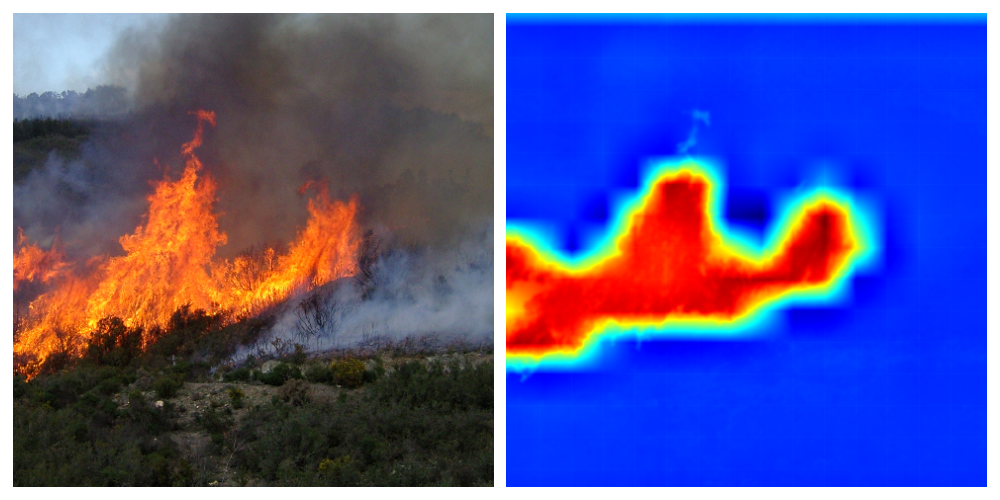
\includegraphics[width=0.5\textwidth]{fig/inferencepic.png}

Wild Fire Watch 
\end{frame}



\begin{frame}{Objetivos}
\begin{itemize}
    \item Reproducción y verificación de SFEwAN. 
    \item Análisis de tiempos. 
    \item Análisis de consumo de energía en plataformas embebidas. 
\end{itemize}
    
\end{frame}

%https://www.terram.cl/2017/03/megaincendio-de-chile-el-mas-intenso-de-la-historia/
\section{Estado del Arte}

\begin{frame}{Redes neuronales}

	\centering
 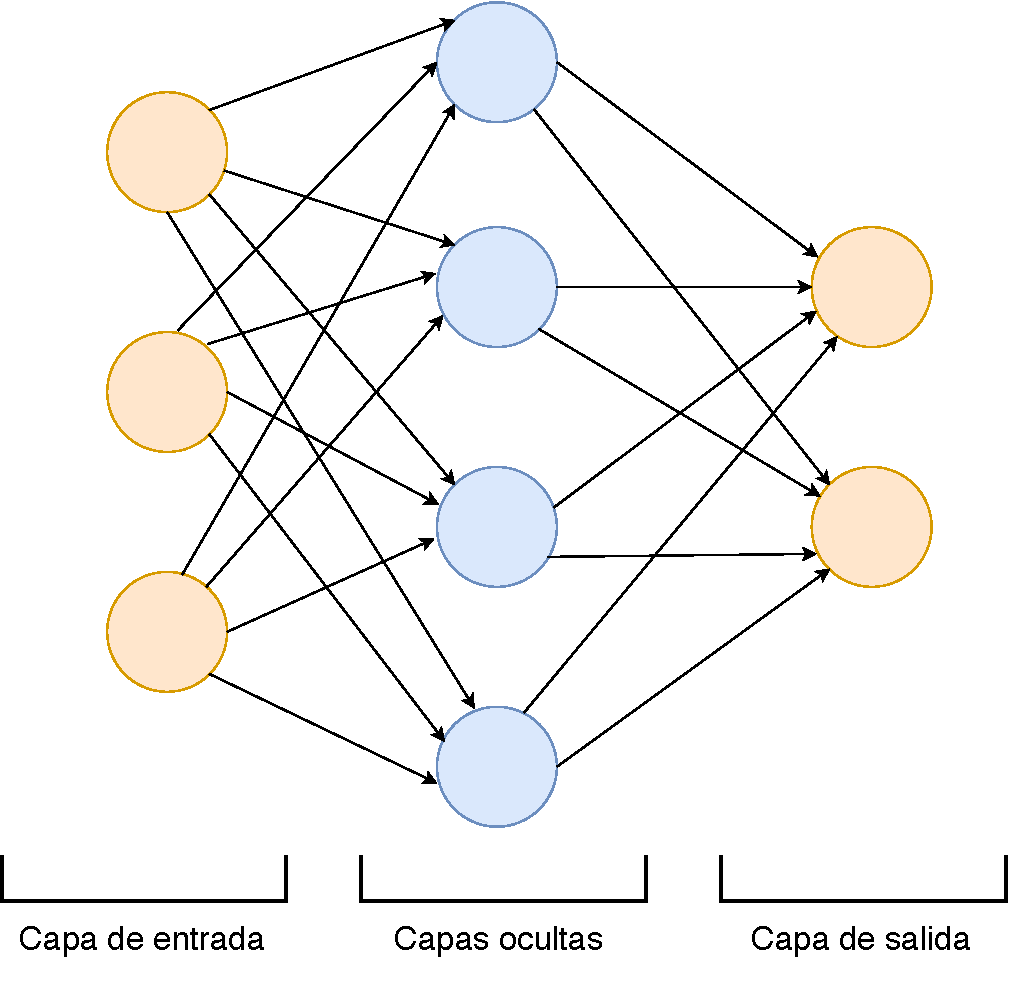
\includegraphics[width=0.5\textwidth]{fig/redneuronal.pdf}

\end{frame}

\begin{frame}{Redes neuronales}
\framesubtitle{FCN AlexNet}

	\centering
 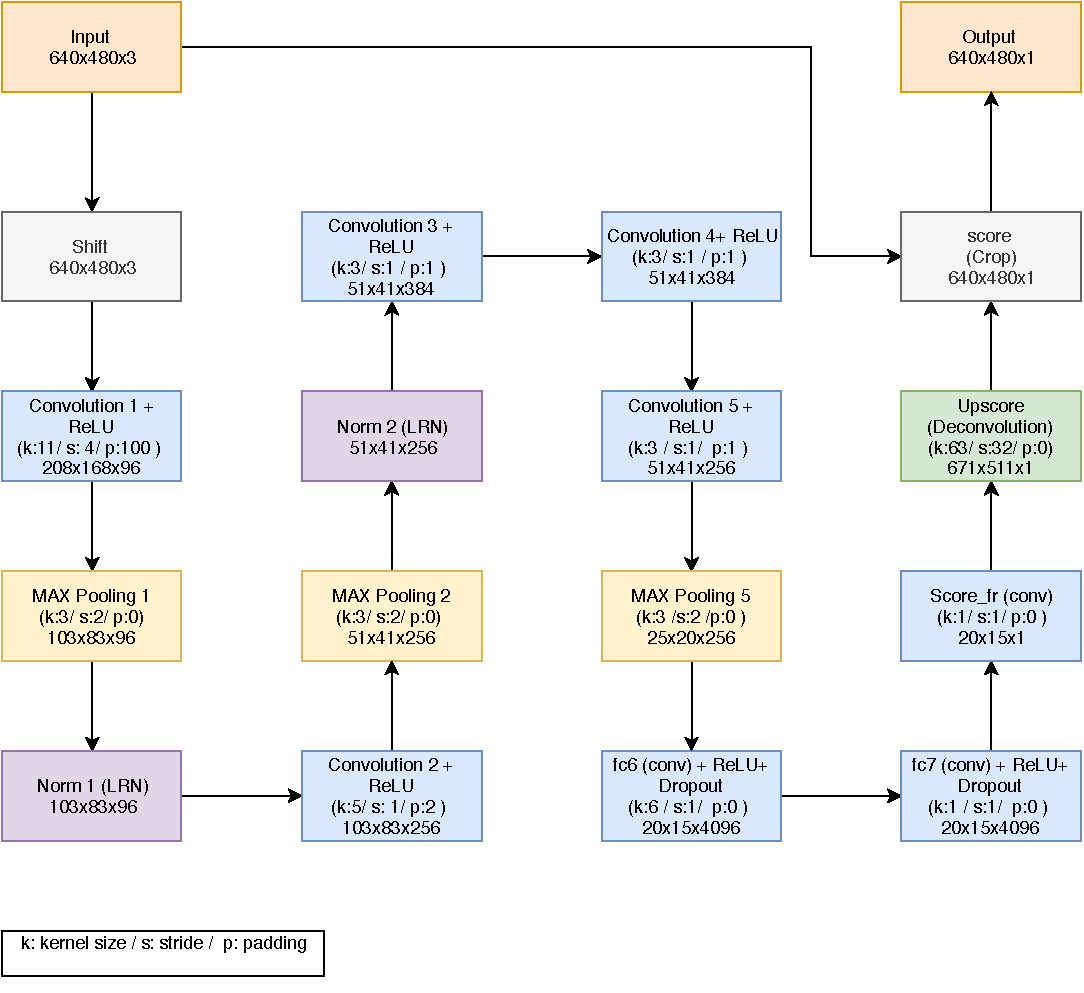
\includegraphics[width=0.7\textwidth]{anexo/FCN-Alex.pdf}
\end{frame}

\begin{frame}{Redes neuronales}
\framesubtitle{Simple Feature Extraction}
	\centering
 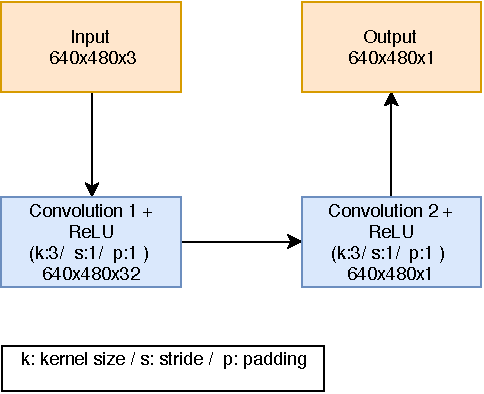
\includegraphics[width=0.4\textwidth]{anexo/sfe.pdf}
\end{frame}

\begin{frame}{Redes neuronales}
\framesubtitle{SFEwAN}
	\centering
 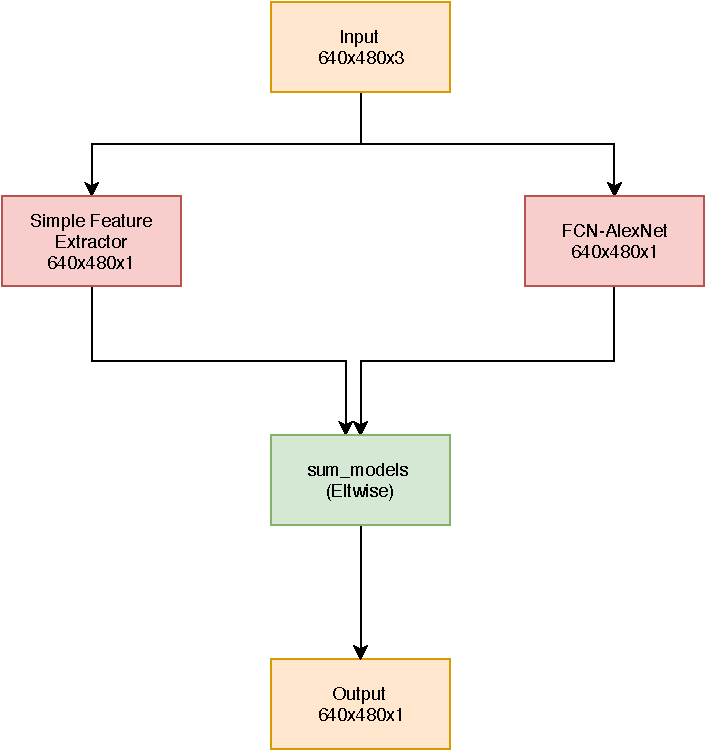
\includegraphics[width=0.6\textwidth]{anexo/sfewan.pdf}
\end{frame}




\begin{frame}{Herramientas de desarrollo para redes neuronales}

	\centering
 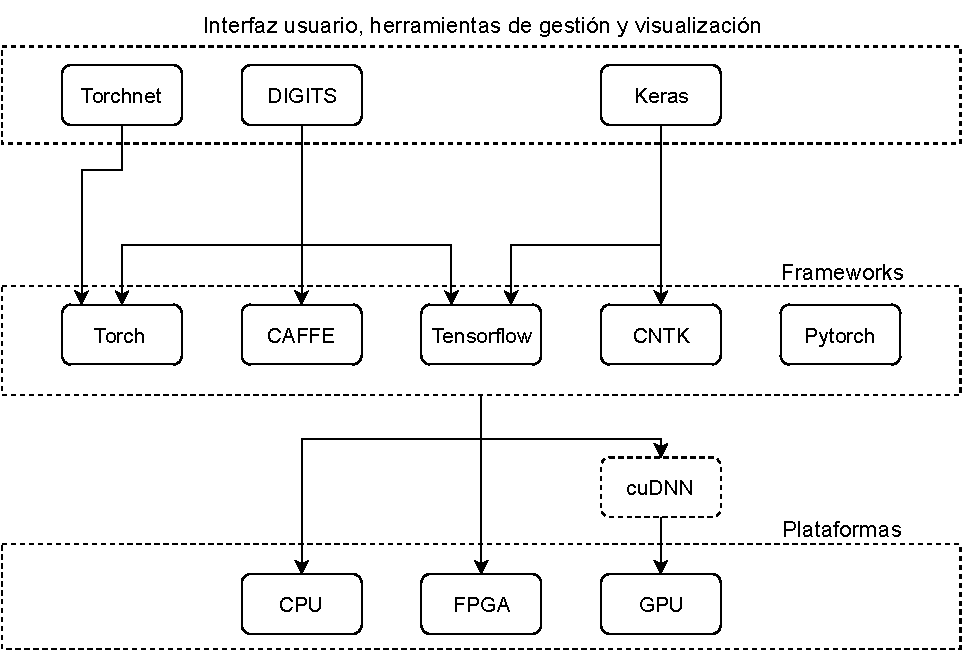
\includegraphics[width=0.9\textwidth]{fig/DL-frameworks.pdf}

\end{frame}


\begin{frame}{Programación paralela}

\centering
 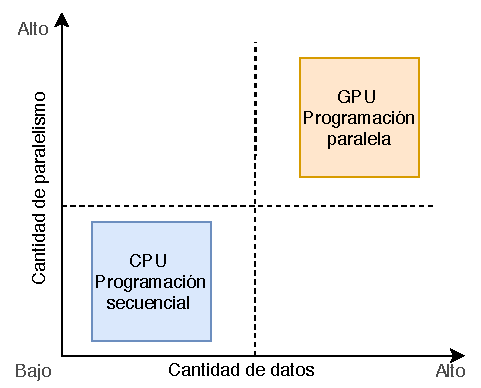
\includegraphics[width=0.6\textwidth]{fig/paralelismo.pdf}

\end{frame}


\begin{frame}{Sistemas basados en GPU}
\resizebox{\linewidth}{!}{% Resize table to fit within \linewidth horizontally
\begin{table}[]
\centering
\begin{tabular}{lccccc}
\toprule
             & Jetson TX2                                                          & Jetson AGX Xavier & Laptop 950M                                                   & Sistema 1080Ti                                                 & Sistema TITAN RTX                                              \\ \midrule
CUDA cores   & 256                                                                 & 512               & 640                                                           & 3584                                                           & 4608                                                           \\
Tensor cores & -                                                                   & 64                & -                                                             & -                                                              & 576                                                            \\
CC           & 6.2                                                                 & 7.2               & 5.0                                                             & 6.0                                                              & 7.5                                                            \\
CPU          & \begin{tabular}[c]{@{}c@{}}Denver 2-core \\ ARM 4-core\end{tabular} & ARM 8-core        & \begin{tabular}[c]{@{}c@{}}Intel core \\ i7-6700\end{tabular} & \begin{tabular}[c]{@{}c@{}}Intel core\\  i5-8600K\end{tabular} & \begin{tabular}[c]{@{}c@{}}Intel core \\ i5-8600K\end{tabular}\\
\bottomrule
\end{tabular}
\end{table}
}
\centering
 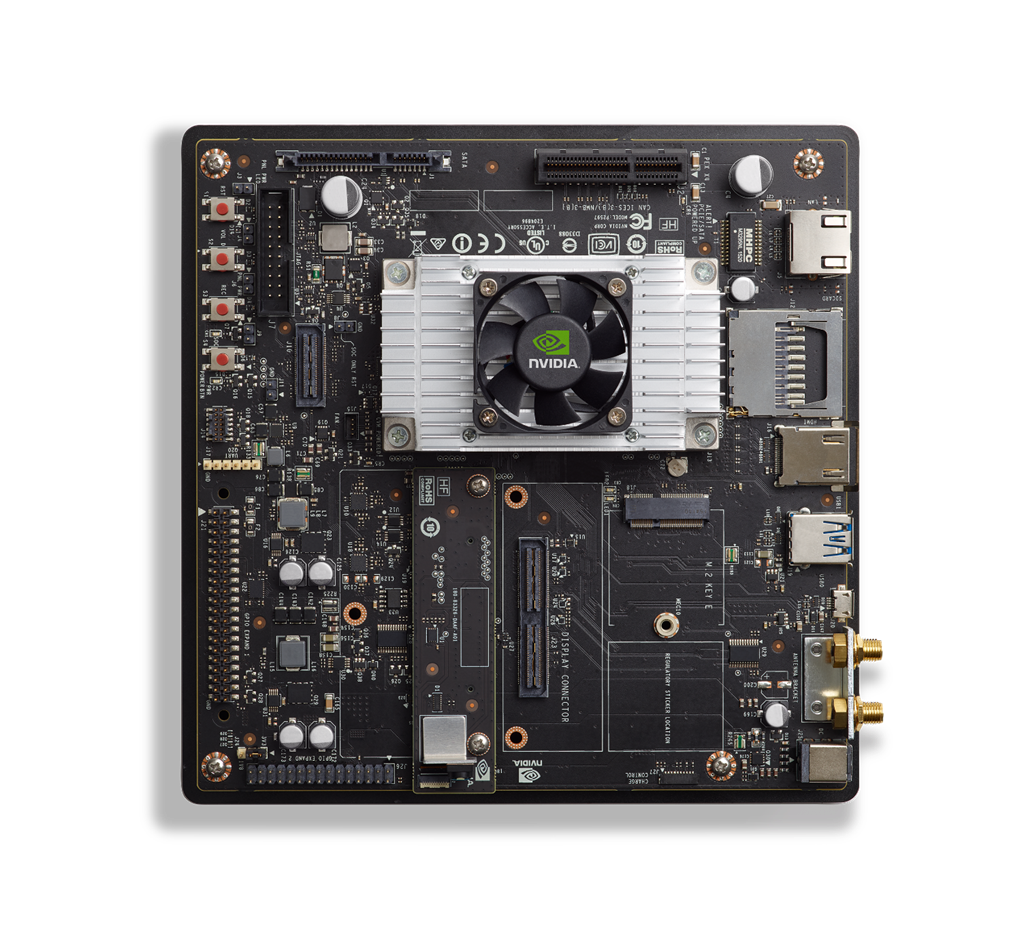
\includegraphics[width=0.3\textwidth]{fig/JTX2.png}
  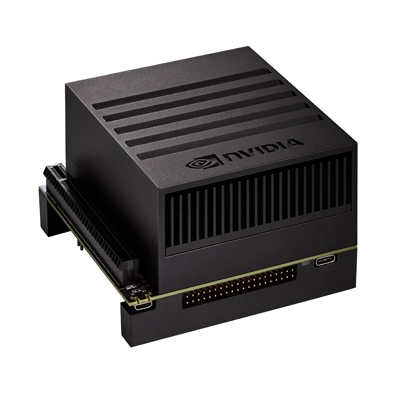
\includegraphics[width=0.25\textwidth]{fig/XAVIER.jpg}
    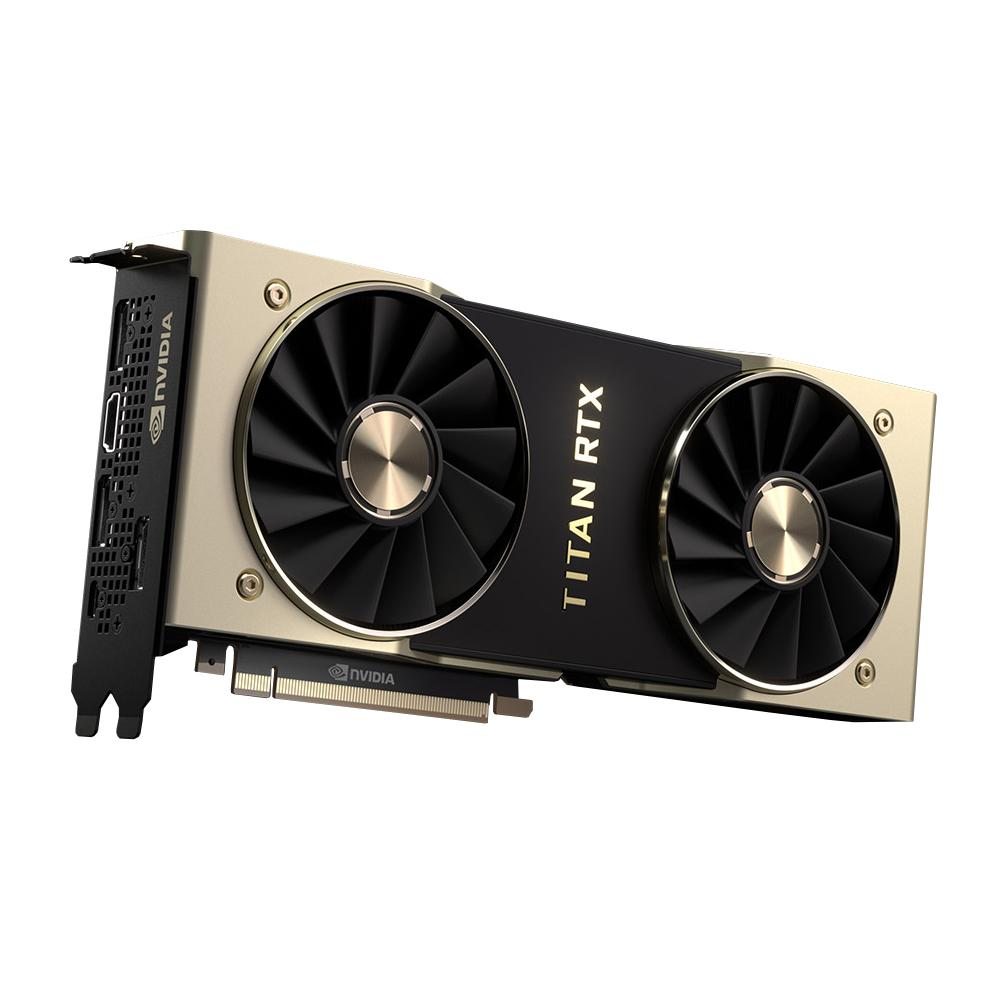
\includegraphics[width=0.3\textwidth]{fig/titan.jpg}
  \end{frame}



\section{Resultados}

\begin{frame}
\centering
\huge
Resultados de tiempo 
    
\end{frame}

\begin{frame}{Tiempos de inferencia}

\framesubtitle{DIGITS}
	\begin{columns}
		\column{.1\textwidth}
 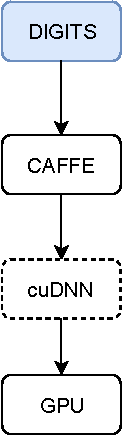
\includegraphics[width=1\textwidth]{diagrama/frame1.pdf}
        
        \column{.85\textwidth}
	\begin{figure}[H]
	\centering
 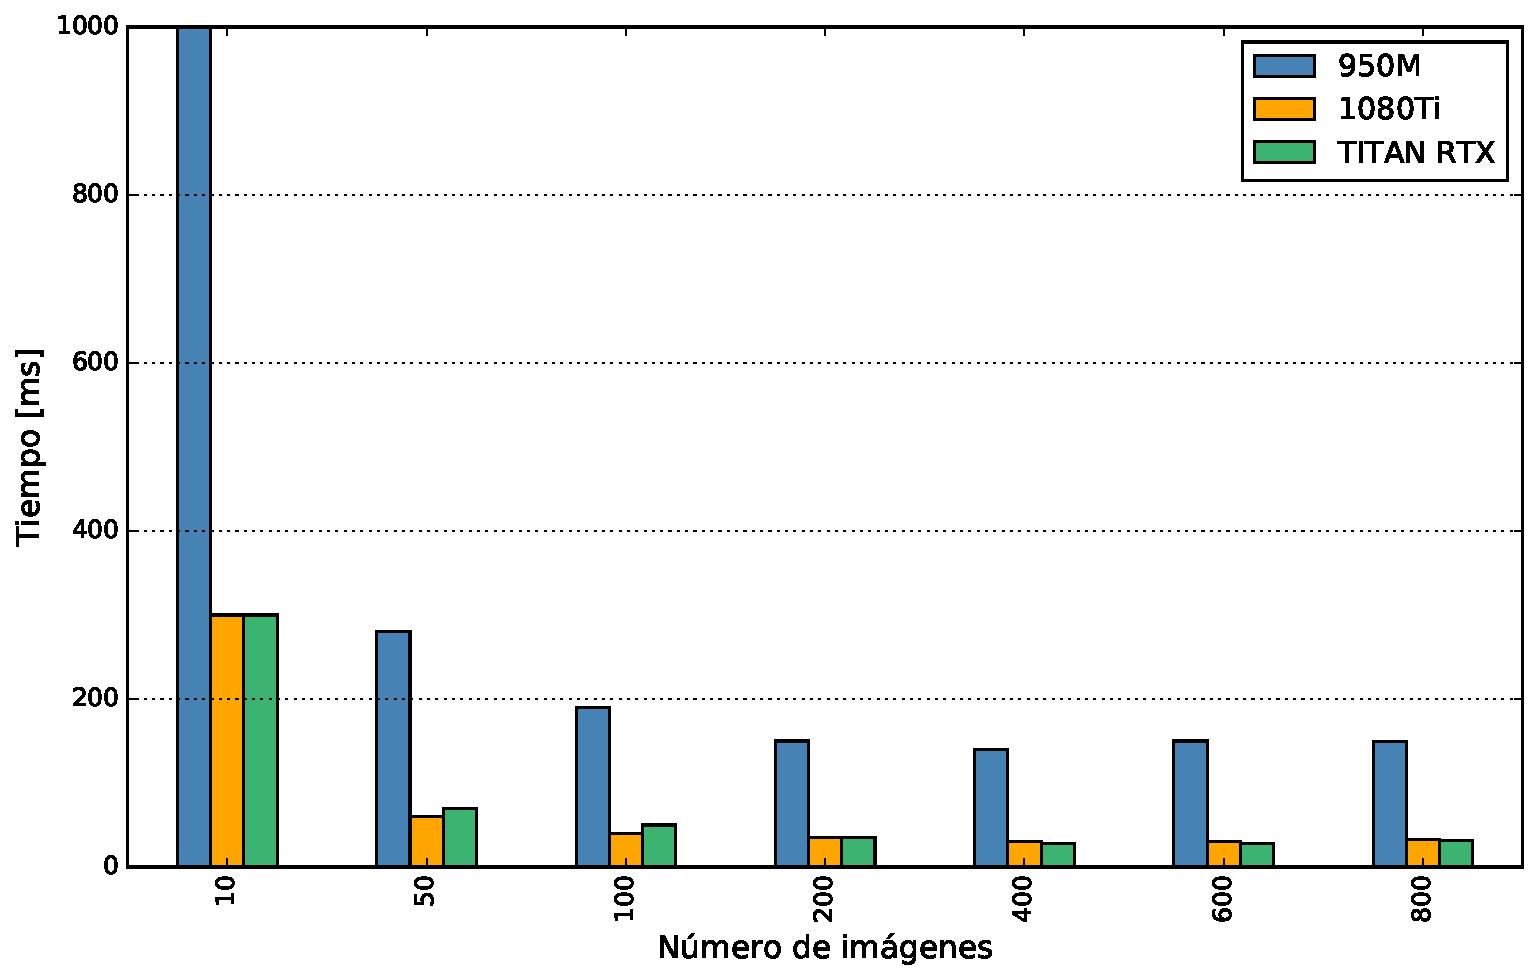
\includegraphics[width=1\textwidth]{barplot/digits.pdf}
	\end{figure}
	\end{columns}
 
\end{frame}



\begin{frame}{Tiempos de inferencia}

\framesubtitle{Caffe}
	\begin{columns}
		\column{.1\textwidth}
 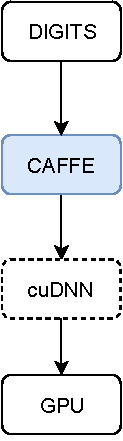
\includegraphics[width=1\textwidth]{diagrama/frame2.pdf}
        
        \column{.85\textwidth}
	\begin{figure}[H]
	\centering
 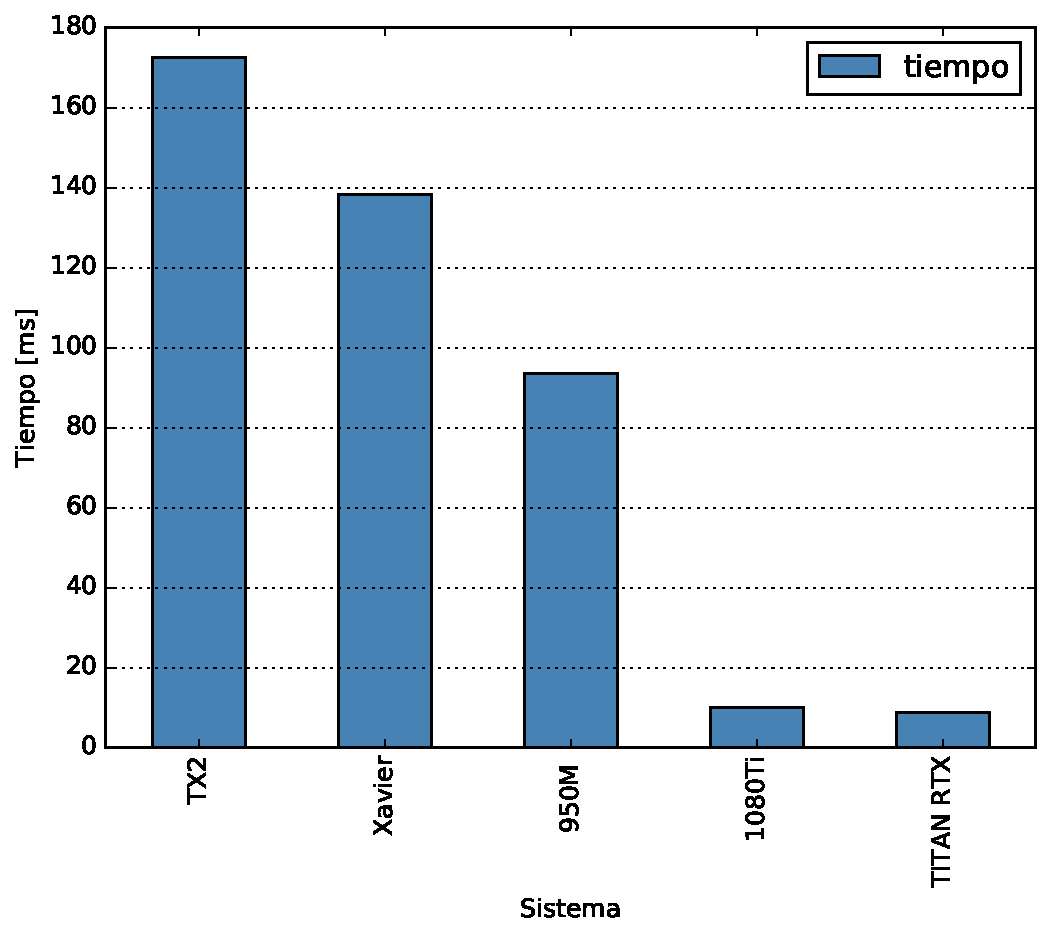
\includegraphics[width=0.7\textwidth]{barplot/avg-fire.pdf}
	\end{figure}
	\end{columns}
 
\end{frame}





\begin{frame}{Tiempos por capa}
\framesubtitle{FCN AlexNet}
	\centering
 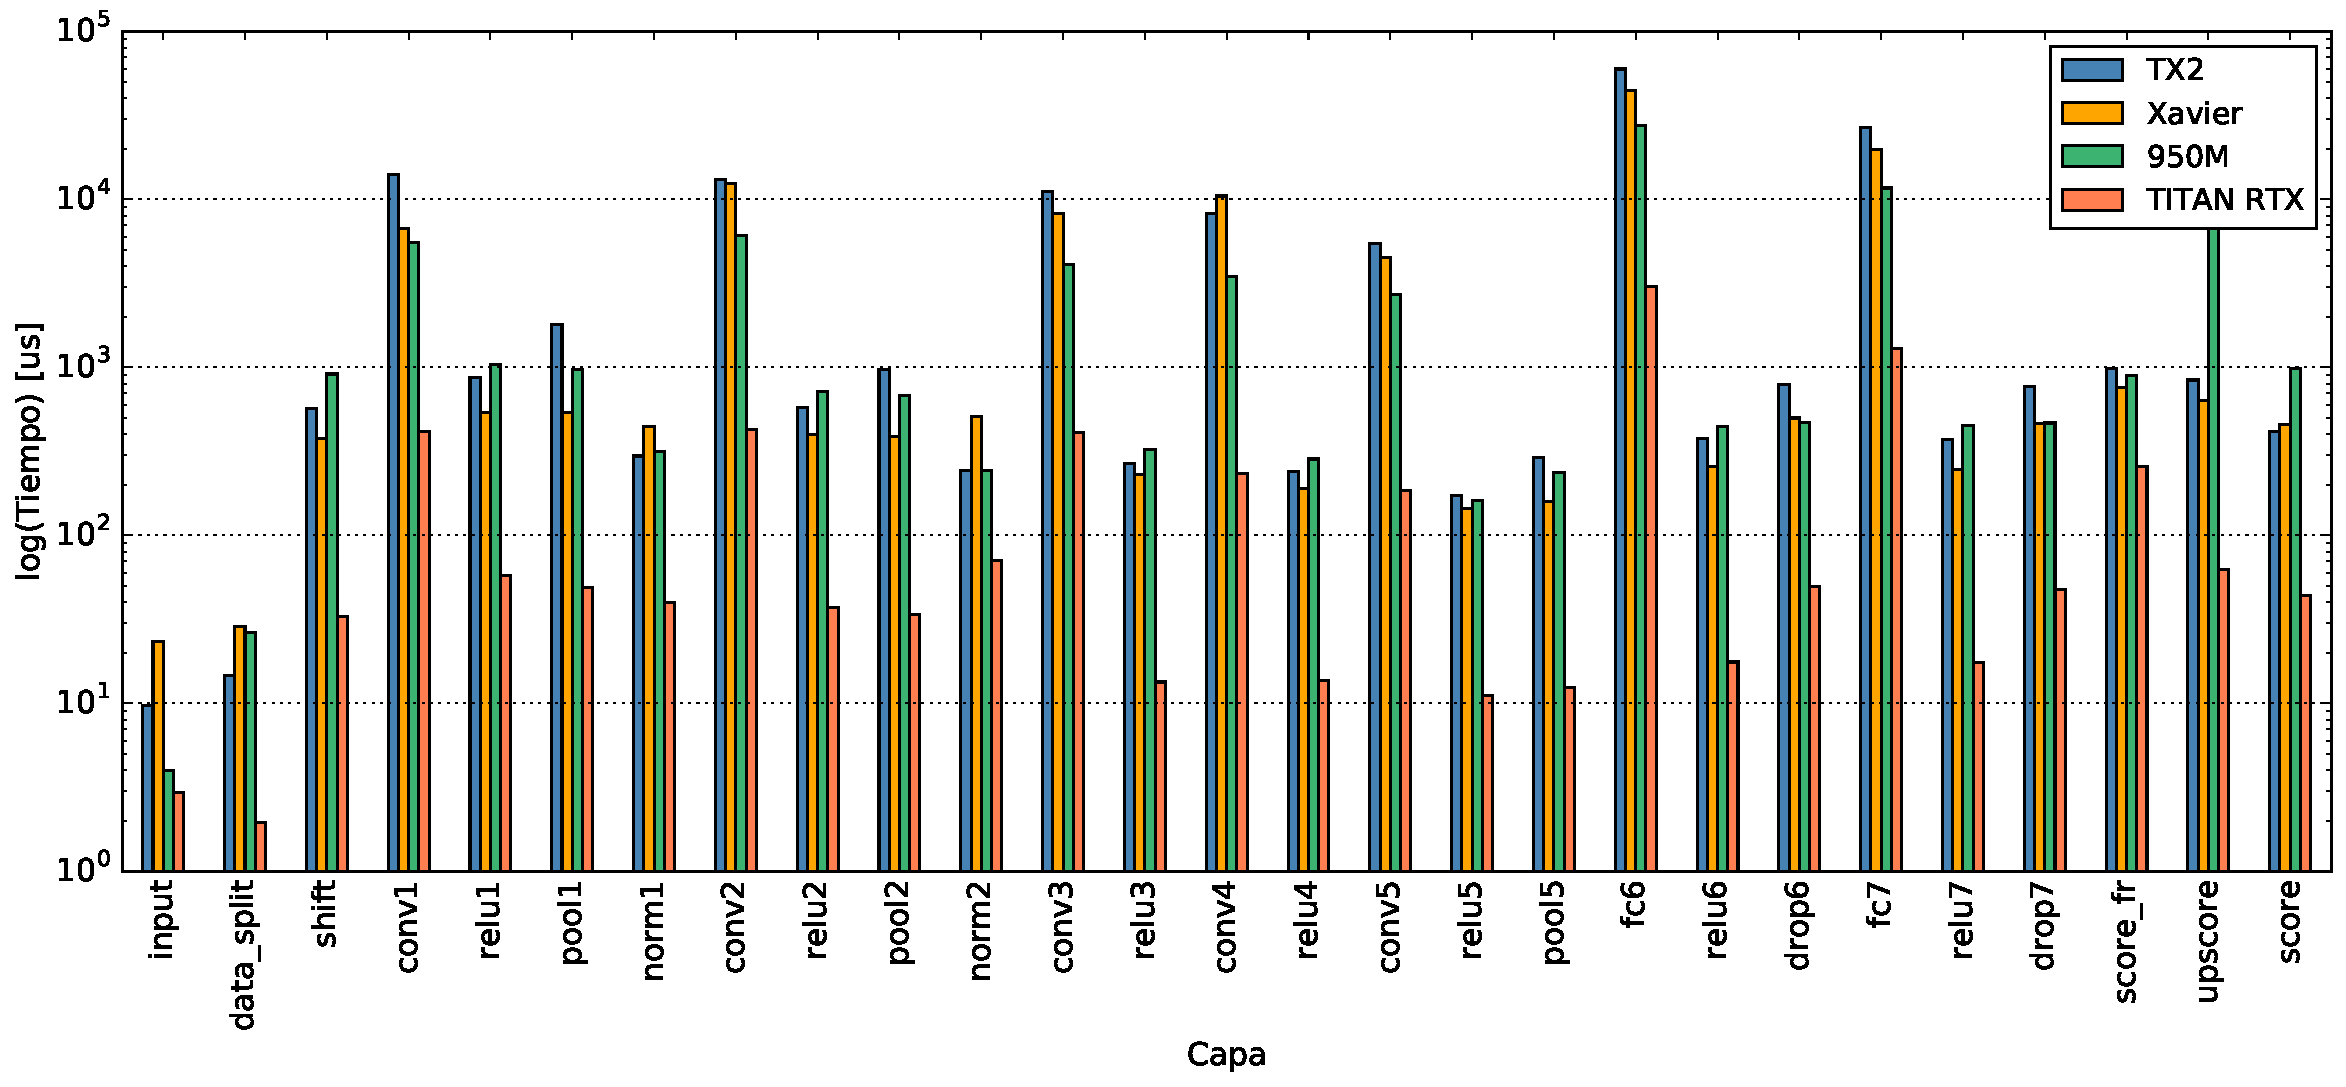
\includegraphics[width=1\textwidth]{barplot/layers-alex.pdf}

\end{frame}

\begin{frame}{Tiempos por capa}
\framesubtitle{Simple Feature Extraction}
	\centering
 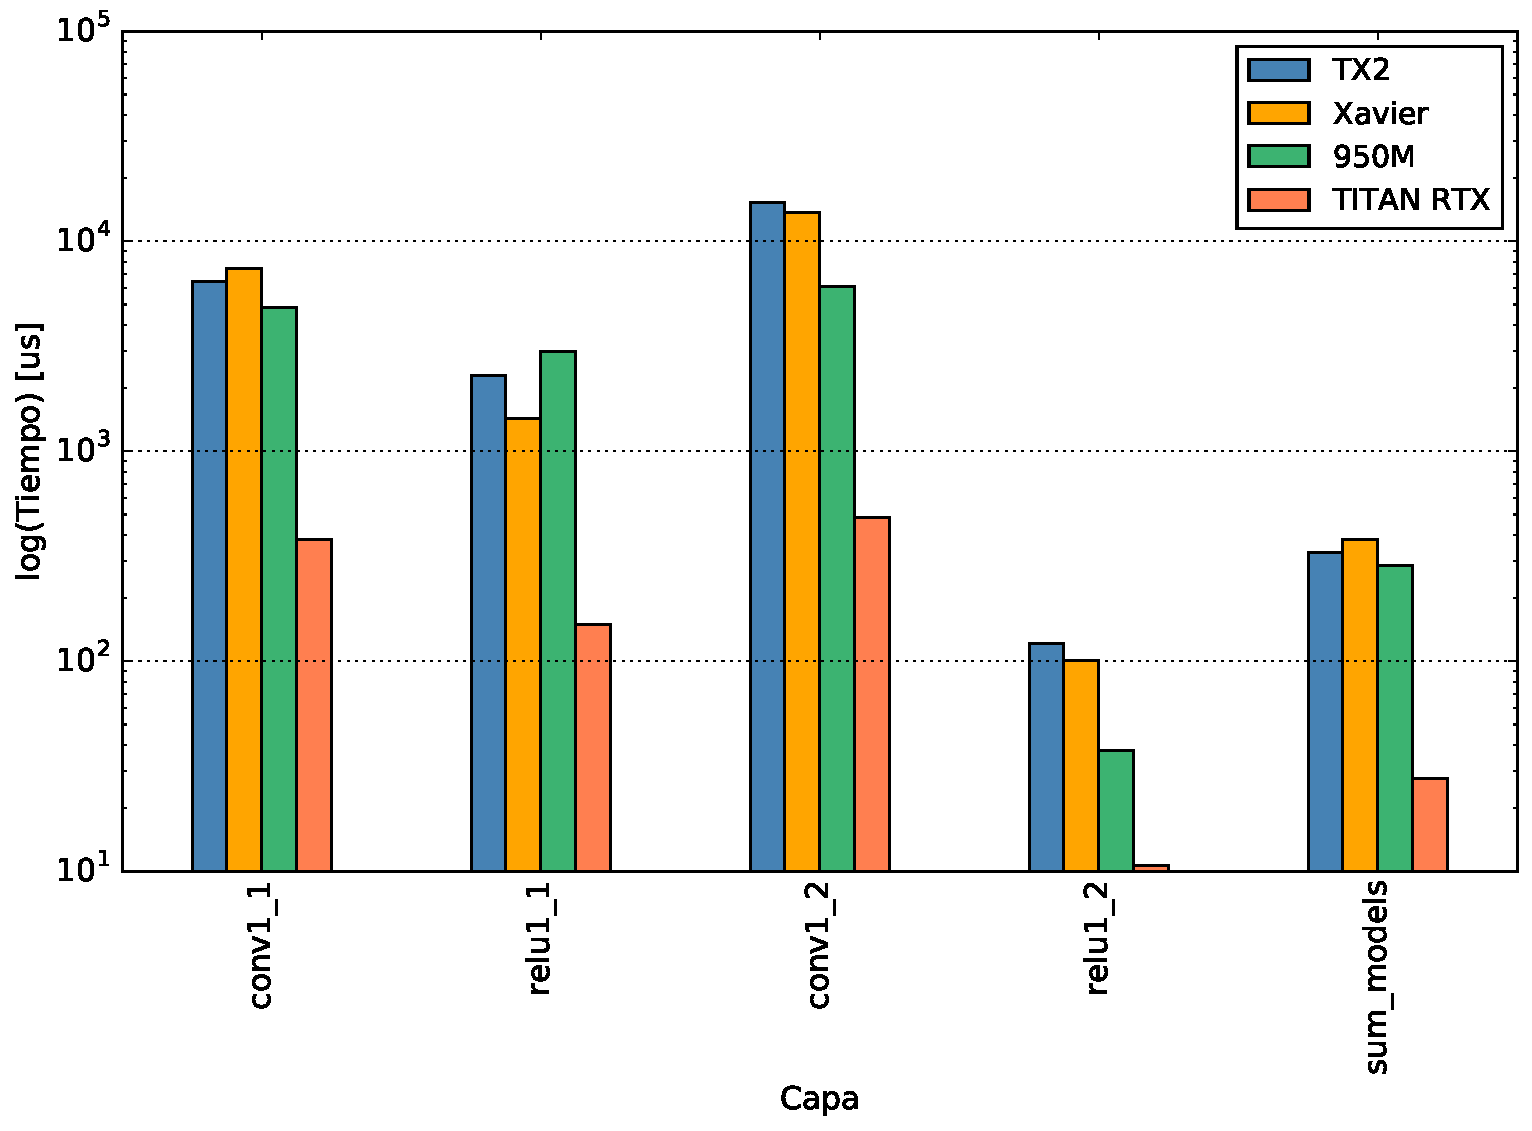
\includegraphics[width=0.7\textwidth]{barplot/layers-sfe.pdf}

\end{frame}



 
\begin{frame}{Tiempos por función}
\framesubtitle{Análisis de dependencias Jetson TX2}
\centering
\resizebox{0.75\linewidth}{!}{


\begin{table}[]
\centering

\begin{tabular}{lcc}
\toprule
Kernel   & Critical path {[}\%{]} & Critical path {[}s{]} \\
\midrule
cuDNN GEMM      & 43.84                  & 39.56                  \\
cuDNN ReLU      & 7.47                   & 6.75                   \\
CPU other & 5.5                    & 4.96                   \\
cuDNN Winograd  & 2.73                   & 2.46       \\
\bottomrule
\end{tabular}

\end{table}
}
\end{frame}


\begin{frame}{Tiempos por función}
\framesubtitle{Análisis de dependencias Jetson AGX Xavier}
\centering
\resizebox{0.75\linewidth}{!}{
\begin{table}[]
\centering

\begin{tabular}{lcc}
\toprule
Kernel      & \multicolumn{1}{l}{Critical path {[}\%{]}} & \multicolumn{1}{l}{Critical path {[}s{]}} \\
\midrule
cuDNN GEMM         & 58.65                                      & 5.47                                      \\
Caffe im2col & 7.7                                        & 0.74                                      \\
CPU other    & 5.84                                       & 0.56                                      \\
Caffe ReLU   & 0.84                                       & 0.08    \\
\bottomrule
\end{tabular}

\end{table}
}
\end{frame}



\begin{frame}{Tiempos por llamada API CUDA}
	\begin{columns}
		\column{.1\textwidth}
 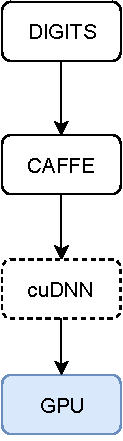
\includegraphics[width=1\textwidth]{diagrama/frame4.pdf}
        
        \column{.85\textwidth}
	\begin{figure}[H]
	\centering
 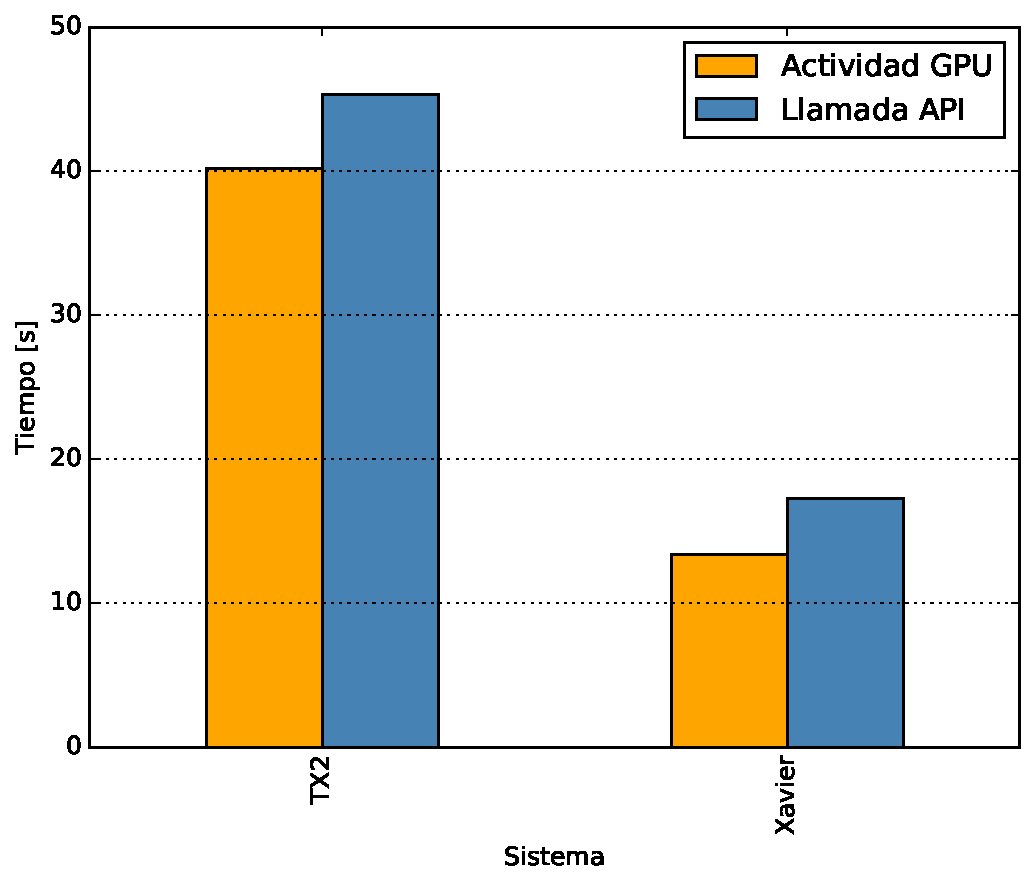
\includegraphics[width=0.7\textwidth]{barplot/gpu-act.pdf}
	\end{figure}
	\end{columns}
\end{frame}
 
\begin{frame}{Tiempos por llamada de API CUDA}
\framesubtitle{Análisis de dependencias Jetson TX2}
\resizebox{\linewidth}{!}{


\begin{table}[]
\centering

\begin{tabular}{lccccc}
\toprule
Llamada API              & Critical path {[}\%{]} & Critical path {[}s{]} & Tiempo espera {[}s{]} \\
\midrule
Stream create with flags & 28.14                  & 25.41                 & 0.00                  \\
cuda Free                 & 1.82                   & 1.64                  & 0.00                  \\
cuda Event Synchronize        & 0.64                   & 0.58                  & 58.58                \\
\bottomrule
\end{tabular}

\end{table}
}
\end{frame}


\begin{frame}{Tiempos por llamada de API CUDA}
\framesubtitle{Análisis de dependencias Jetson AGX Xavier}
\resizebox{\linewidth}{!}{
\begin{table}[]
\centering

\begin{tabular}{lccc}
\toprule
Llamada API   & Critical path {[}\%{]} & Critical path {[}s{]} & Tiempo espera {[}s{]} \\
\midrule
cuda Free      & 15.91                  & 1.53                  & 0.00                  \\
cuda Malloc    & 0.66                   & 0.63                  & 0.00                  \\
cuda Event Synchronize & 0.42                   & 0.04                  & 3.35                 \\
\bottomrule
\end{tabular}

\end{table}
}
\end{frame}




\begin{frame}
\centering
\huge
Resultados de consumo de energía
    
\end{frame}


\begin{frame}{Consumo de energía: Jetson TX2}
\centering
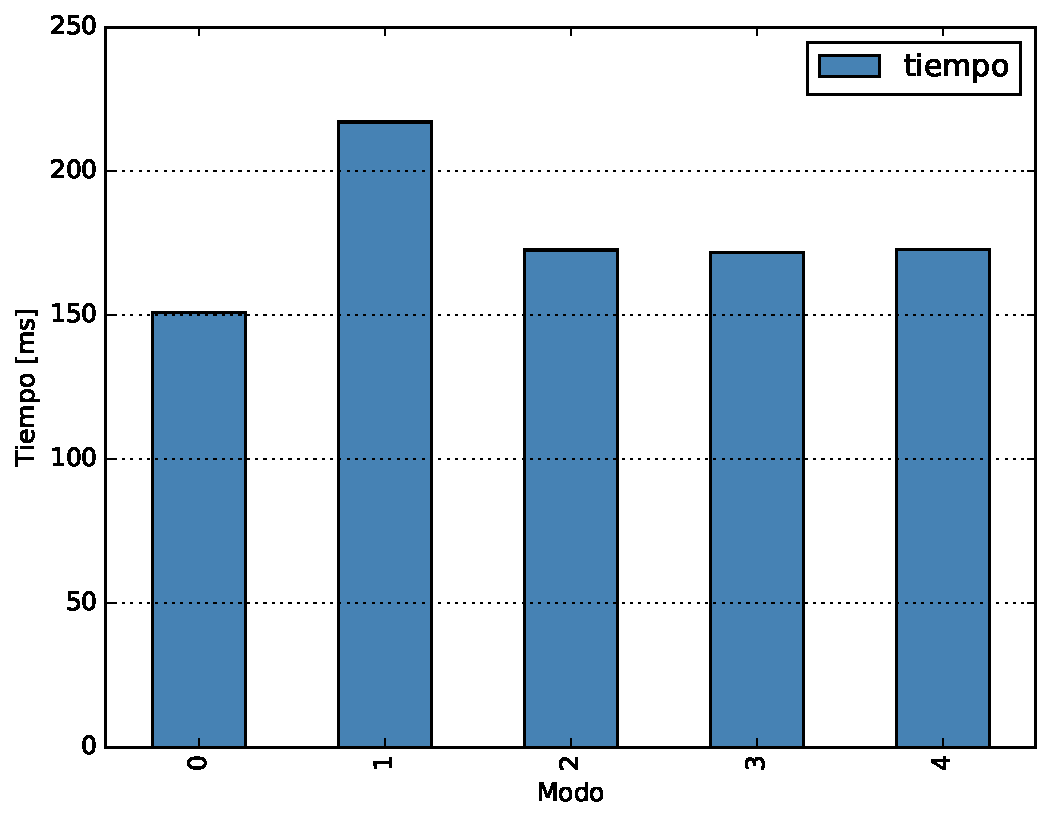
\includegraphics[width=0.7\textwidth]{barplot/modes-ttx2.pdf}
\end{frame}

\begin{frame}{Consumo de energía: Jetson TX2}
\centering
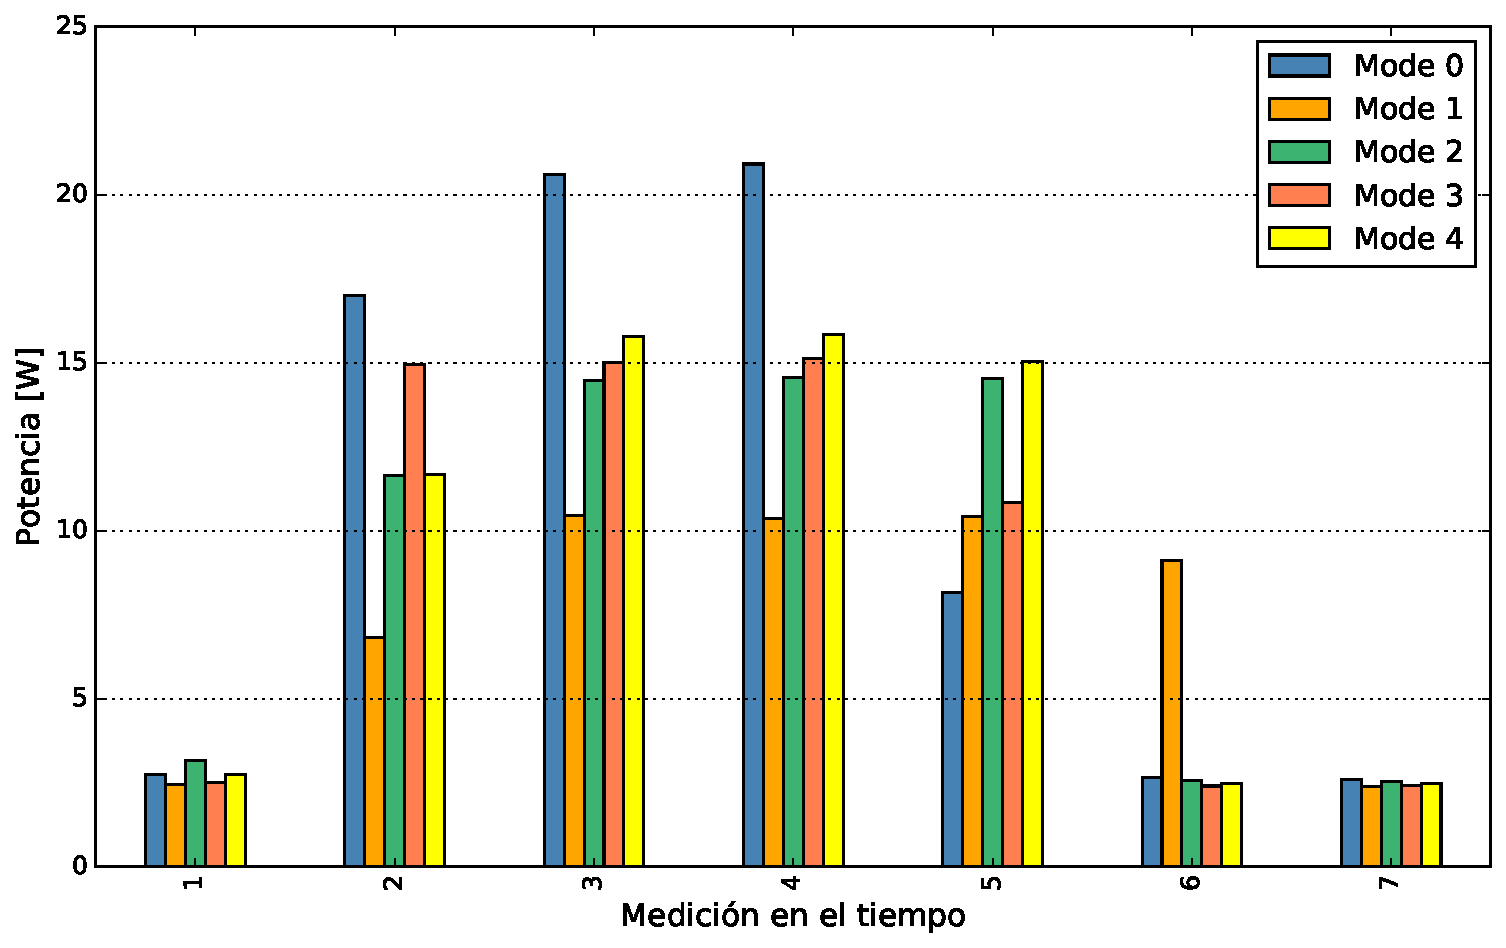
\includegraphics[width=0.9\textwidth]{barplot/power-tx2.pdf}
\end{frame}



\begin{frame}{Consumo de energía: Jetson AGX Xavier}

\centering
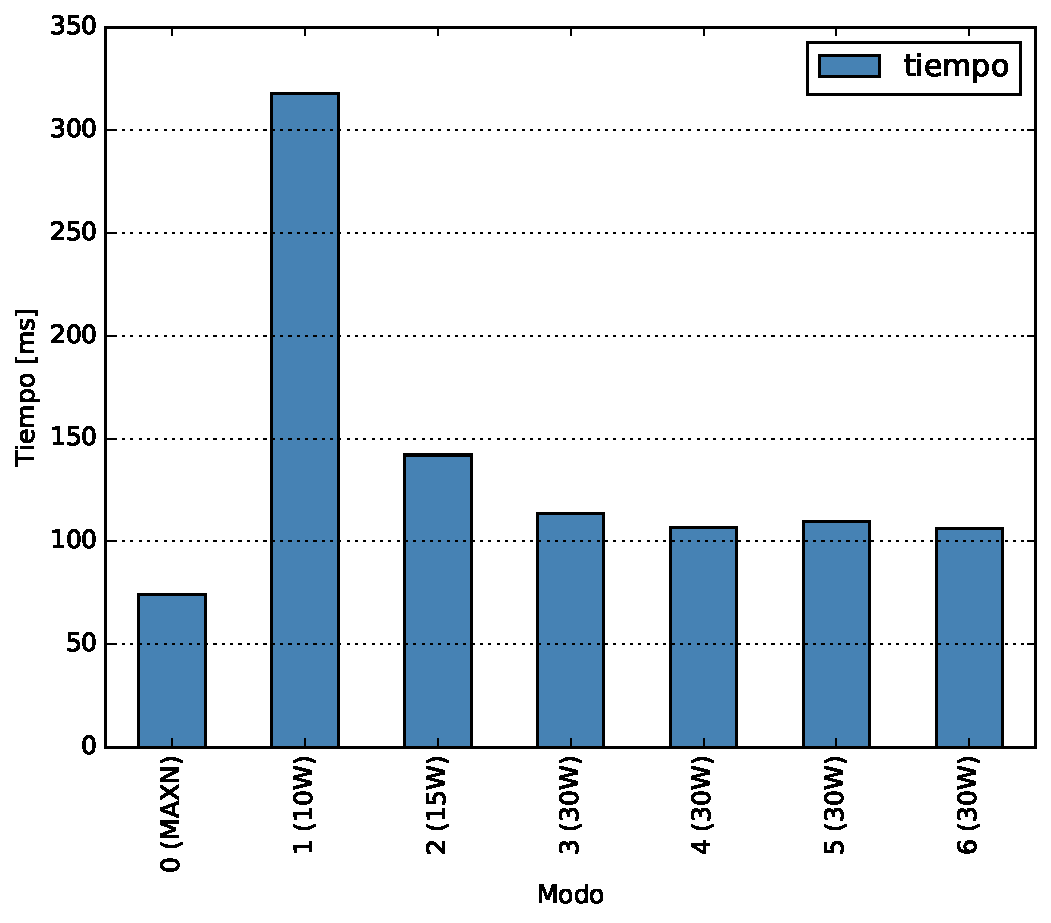
\includegraphics[width=0.7\textwidth]{barplot/modes-txavier.pdf}

\end{frame}

\begin{frame}{Consumo de energía: Jetson AGX Xavier}

\centering
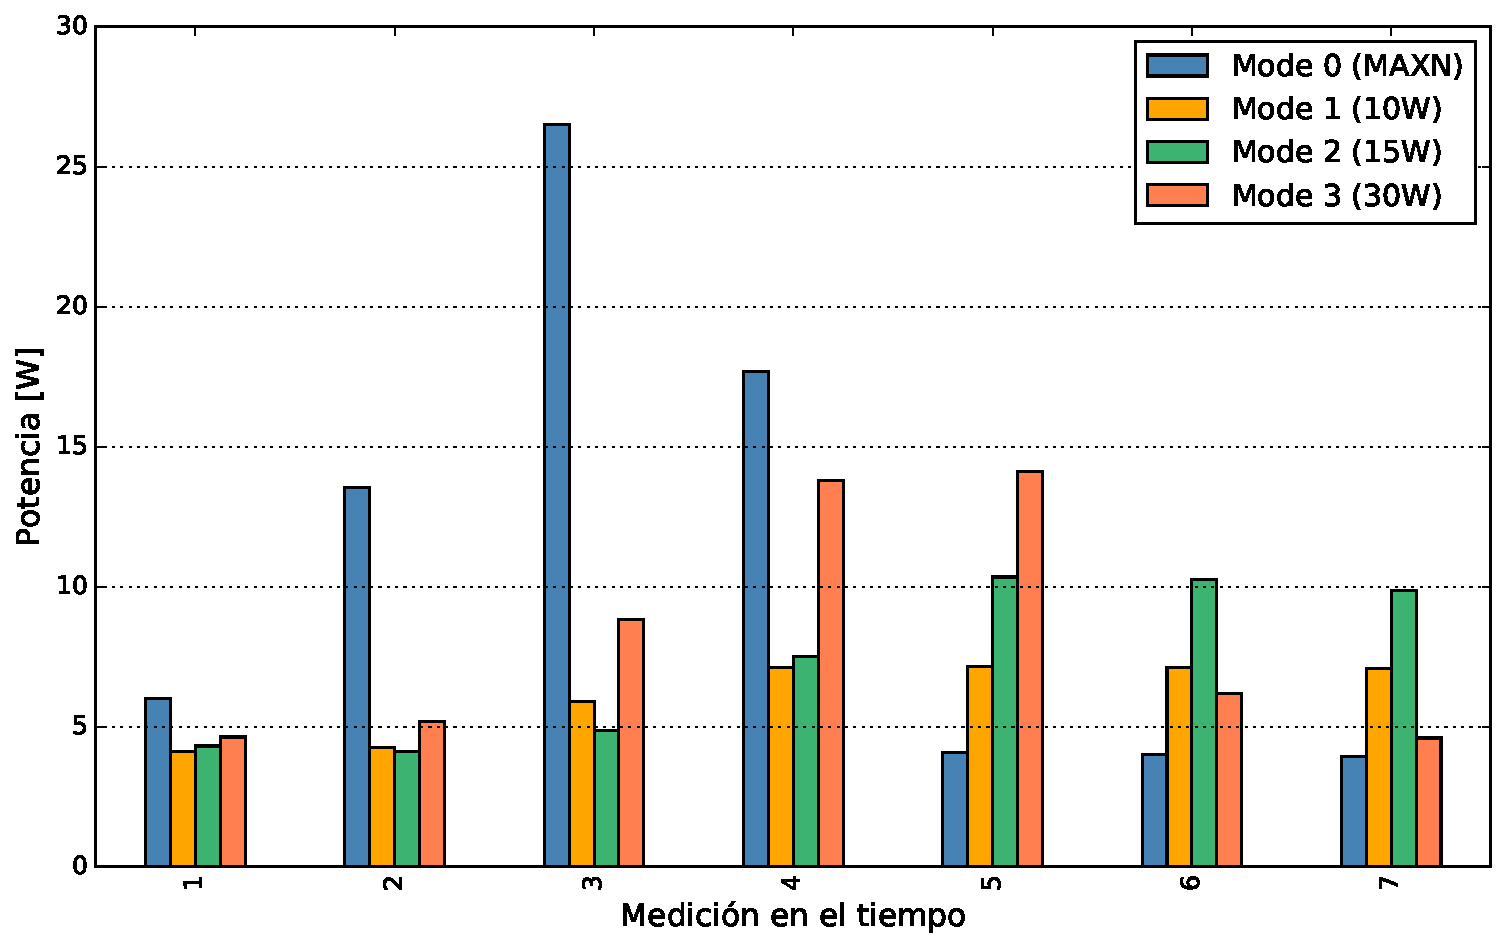
\includegraphics[width=0.9\textwidth]{barplot/power-xavier.pdf}
\end{frame}


\begin{frame}{Consumo de energía: 1080Ti y TITAN RTX}

\centering
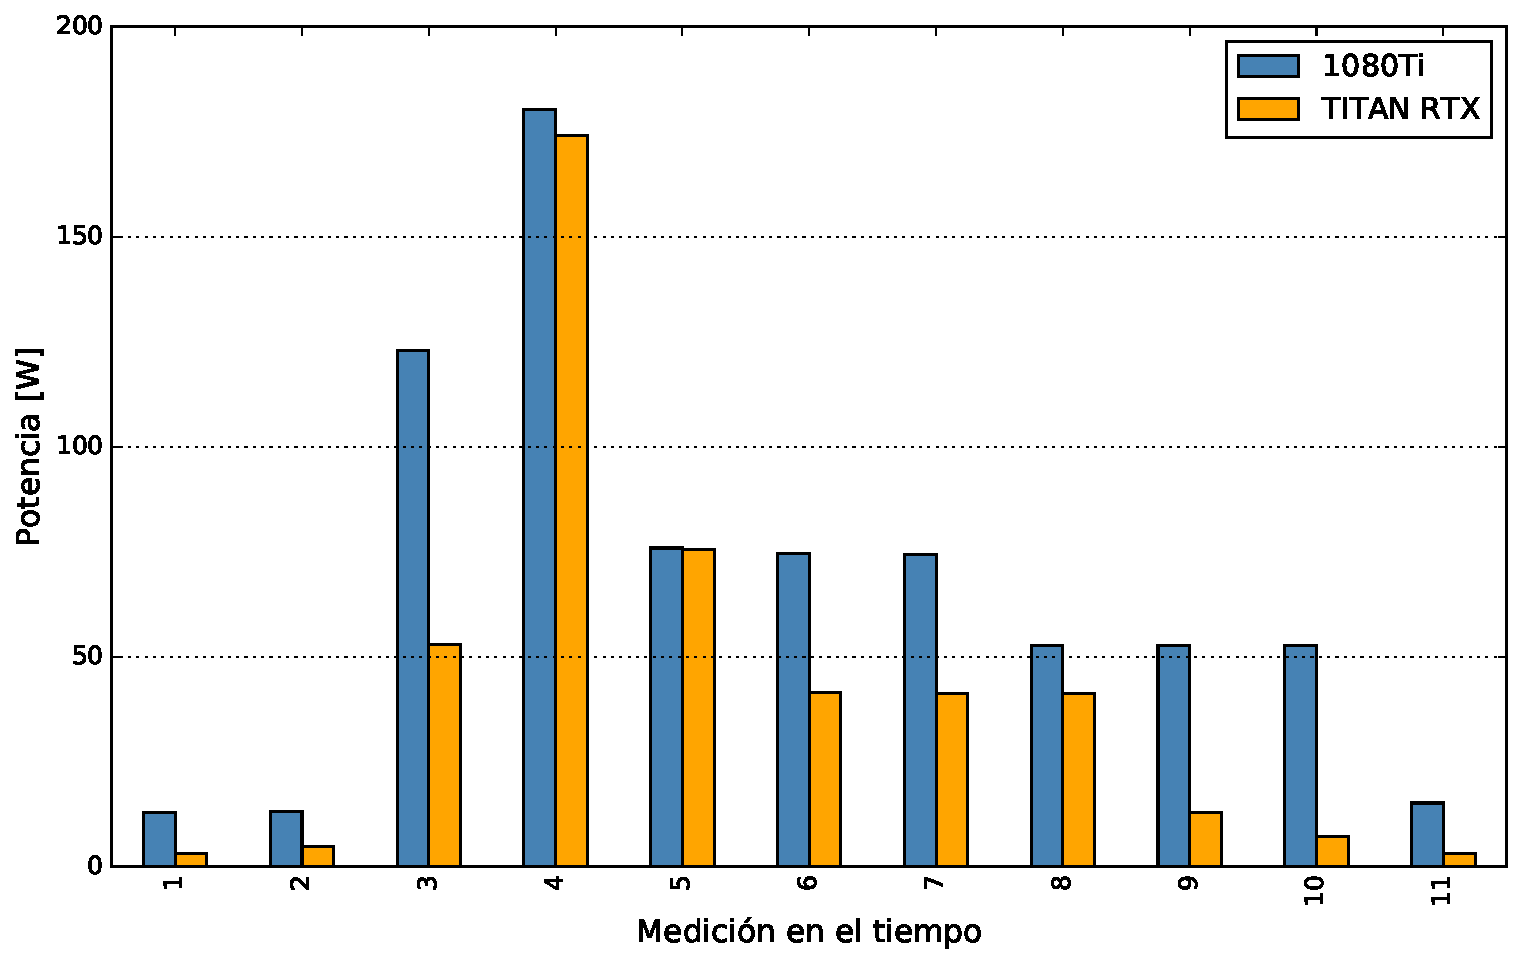
\includegraphics[width=1\textwidth]{barplot/TITAN-1080.pdf}

\end{frame}


\begin{frame}
\centering
\huge
Comparación frameworks
\end{frame}

\begin{frame}{Comparación de frameworks}

  \newline
\centering
\resizebox{0.6\linewidth}{!}{
\begin{table}[]
\begin{tabular}{lcc}
\toprule
                 & Tensorflow    & Caffe         \\
                 \midrule
Tiempo ejecución & 5.711 {[}s{]} & 1.586 {[}s{]} \\
Memoria GPU      & 65\%          & 56\%   \\
\bottomrule
\end{tabular}
\end{table}
}

\end{frame}

\begin{frame}{Comparación de frameworks}

\centering
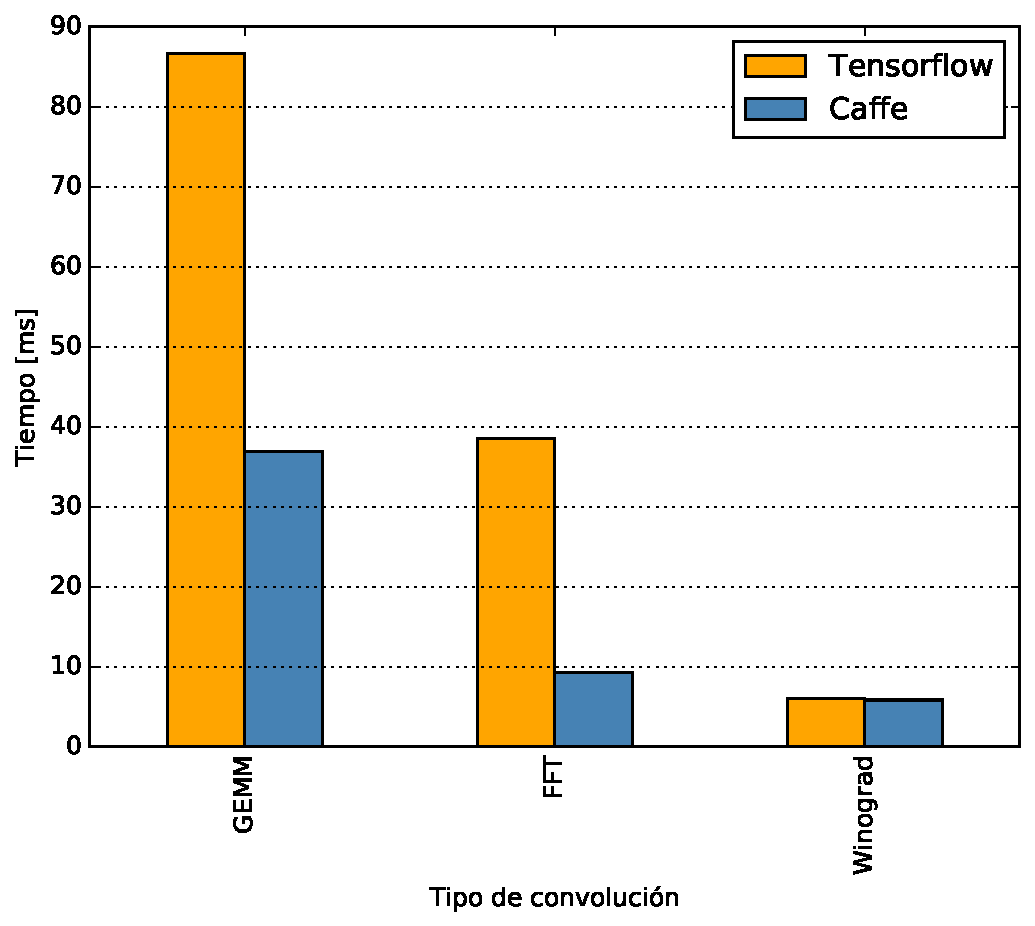
\includegraphics[width=0.5\textwidth]{barplot/tfc-conv.pdf}

\end{frame}
\section{Conclusión}

\begin{frame}{Conclusiones}
\begin{itemize}
    \item  Tasa de inferencia promedio de  5 [fps] y 7 [fps] para los sistemas Jetson TX2 y Jetson AGX Xavier.
    \item  TITAN RTX posee una tasa promedio de 115 [fps]. 

    \item Diferencia de más de un 40\%  entre los modos de mayor y menor consumo dentro un mismo sistema Jetson.
    \item Mejora de rendimiento que han demostrado los sistemas embebidos de Nvidia en un periodo de 20 meses. 
\end{itemize}


\end{frame}


\begin{frame}{Conclusiones}
\centering
Fin.
\end{frame}


\begin{frame}[noframenumbering]{Apéndice}

\framesubtitle{Vista organizacional GPU}
\centering
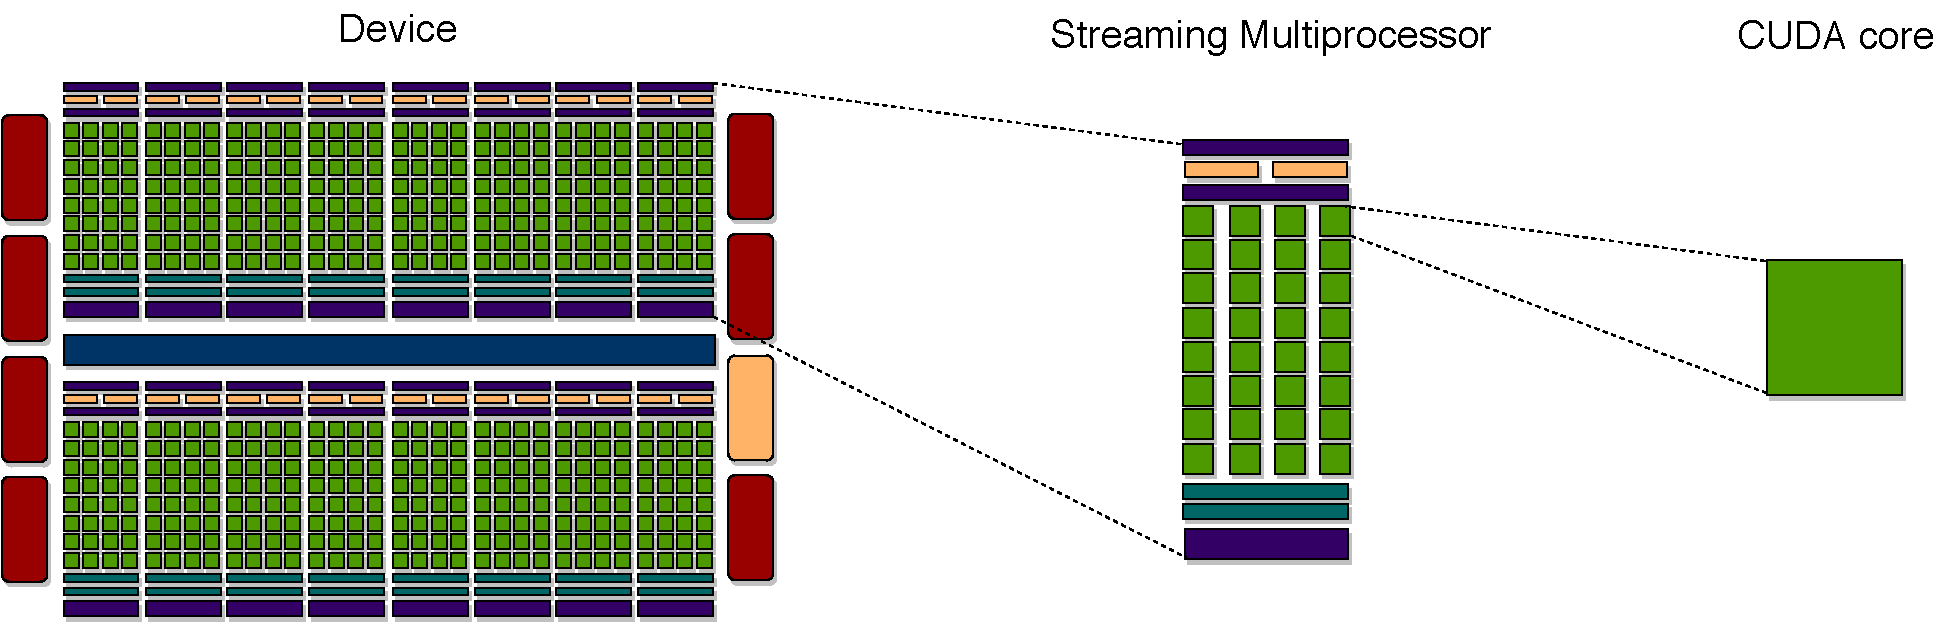
\includegraphics[width=0.9\textwidth]{fig/GPU-diagram1.pdf}

\end{frame}
\begin{frame}[noframenumbering]{Apéndice}
\framesubtitle{Arquitectura LeNet}

\centering
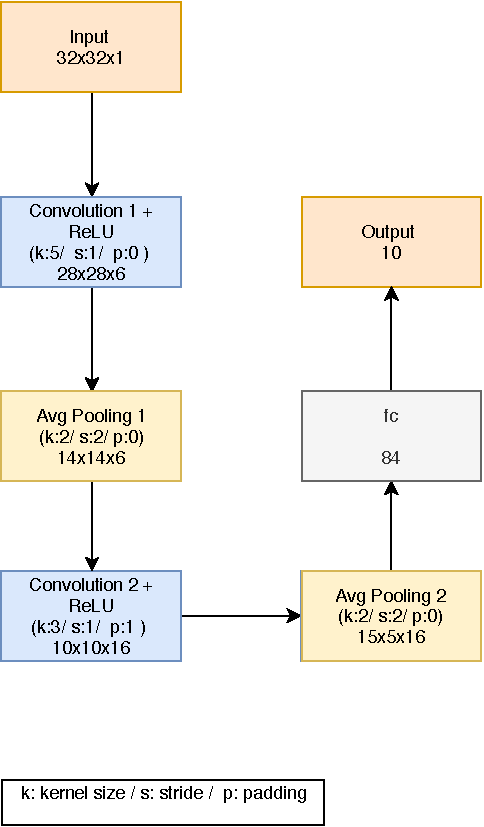
\includegraphics[width=0.35\textwidth]{anexo/lenet.pdf}

\end{frame}
\begin{frame}[noframenumbering]{Apéndice}
\framesubtitle{Modos de energía Jetson TX2}
\centering
\resizebox{0.9\linewidth}{!}{


\begin{table}[]
\centering

\begin{tabular}{lccccc}
\toprule
Modo                     & 0 & 1  & 2     & 3 & 4   \\ \midrule
Nombre                  & Max-N      & Max-Q      & Max-P Core-All & Max-P ARM  & Max-P Denver \\ 
Denver 2                & 2          & 0          & 2              & 0          & 1            \\ 
Frecuencia {[}GHz{]}     & 2          & -          & 1.4            & -          & 2            \\ 
ARM A57                  & 4          & 4          & 4              & 4          & 1            \\ 
Frec. {[}GHz{]}     & 2.0        & 1.2        & 1.4            & 2          & 0.3          \\ 
Frec. GPU {[}GHz{]} & 1.3        & 0.85       & 1.12           & 1.12       & 1.12         \\ 
\bottomrule
\end{tabular}

\end{table}
}

\end{frame}


\begin{frame}[noframenumbering]{Apéndice}
\framesubtitle{Modos de energía Jetson AGX Xavier}
\centering
\resizebox{0.9\linewidth}{!}{



\begin{table}[]

\centering
\begin{tabular}{lccccccc}
\toprule
Modo                      & 0 & 1 & 2 & 3 & 4 & 5 & 6 \\ \midrule
Power budget {[}W{]}      & n/a        & 10         & 15         & 30         & 30         & 30         & 30         \\ 
Num CPUs                    & 8          & 2          & 4          & 8          & 6          & 4          & 2          \\ 
Max freq CPU {[}MHz{]}    & 2265.6     & 1200       & 1200       & 1200       & 1450       & 1780       & 2100       \\ 
GPU TPC                   & 4          & 2          & 4          & 4          & 4          & 4          & 4          \\ 
Max freq GPU {[}MHz{]}    & 1337       & 520        & 670        & 900        & 900        & 900        & 900        \\ 
DLA Cores                 & 2          & 2          & 2          & 2          & 2          & 2          & 2          \\ 
Max freq DLA {[}MHz{]}    & 1395.2     & 550        & 750        & 1050       & 1050       & 1050       & 1050       \\ 
VA cores                  & 2          & -          & 1          & 1          & 1          & 1          & 1          \\ 
Max freq VA {[}MHz{]}     & 1088       & -          & 500        & 760        & 760        & 760        & 760        \\ 
Max freq Memory {[}MHz{]} & 2133       & 1066       & 1333       & 1600       & 1600       & 1600       & 1600       \\ 
\bottomrule
\end{tabular}

\end{table}
}
\end{frame}

\begin{frame}[noframenumbering]{Apéndice}
\framesubtitle{Trabajo Futuro}

\begin{itemize}
    \item Revisar optimizaciones para los sistemas Jetson con TensorRT de Nvidia. 
    \item Optimizaciones a nivel de funciones de cuDNN, con herramientas como $\mu$-cuDNN. 
     \item Realizar una evaluación más profunda del consumo de energía en los sistemas Jetson, considerando las limitaciones de las baterías que alimentan el sistema total, es decir, incluyendo dron y periféricos necesarios.
\end{itemize}
\end{frame}






\end{document}